\subsection{Robotik Systeme} % (fold)
\label{sub:Robotik Systeme}

Roboter kommen immer mehr in Bereichen der Industrie und Haushalt zum Einsatz. Dafür essentiell ist ein System, welches Abstraktionen für die Roboter Systeme bereitstellt und die Konnektivität zwischen den Roboter Schnittstellen herstellt. Eine wichtige Voraussetzung für ein möglicher Standard ist die Unterstützung möglichst vieler Systeme. Die Bandbreite unterschiedlicher Systemen ist mit einfachen embedded Systemen, Industrie Roboter oder Systeme für Selbstfahrende Fahrzeuge sehr Breitgefächert.\\
Mit dem \acrlong{ros} (ROS) der Open Source Robotics Foundation (OSRF) wurde dabei ein System entwickelt, welches die oberen Voraussetzungen erfüllt und sich unter den Robotik Systemen als Standard etabliert hat. Im folgenden wird ROS und die dessen weiterentwicklung ROS 2 vorgestellt. Da im Kontext dieser Arbeit die Kommunikation zwischen Cloud, Edge und Robotik Systemen im Vordergrund steht, werden ebenfalls die Protokolle betrachtet die den Austausch zwischen den verschiedenen Systemen unter sich ermöglichen.

\subsubsection{ROS 2} % (fold)
\label{ssub:ROS 2}

ROS \cite{ConceptsROSDocumentation} ist ein Betriebssystem das verschiedene Arten von Robotern unterstützt. ROS2 ist dabei die zweite Version des Betriebssystems und bringt zahlreiche Änderungen im Aufbau der Komponenten mit sich. Es bietet verschiedene Abstraktionen von Sensoren oder Entwicklungswerkzeige mit sich die wichtig bei der Arbeit im Robotik Bereich sind.\\
ROS hatte zahlreiche Nachteile die als Motivation für die Entwicklung von ROS2 dienten \cite{maruyamaExploringPerformanceROS22016}. Zum einen läuft ROS nur auf Linux und verbraucht viele Ressourcen. Zum anderen und viel wichtiger jedoch, unterstützt es keine Echtzeit Anwendungen \cite{ConceptsROSDocumentation}. Dazu kommt die schlechte Fehlertoleranz und Prozess Synchronisation.\\
ROS2 verbessert die oben genannten Aspekte in dem es eine vollkommen neue Architektur einführt.

\begin{figure}
  \centering
  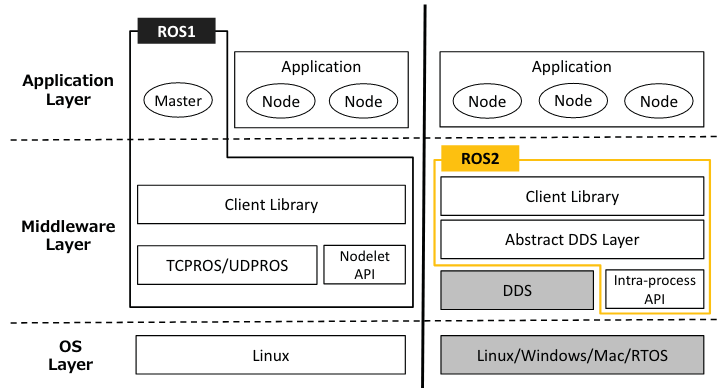
\includegraphics[width=0.95\textwidth]{./figures/ros2-architecture.png}
  \caption{Vergleich der ROS und ROS2 Architektur \cite{maruyamaExploringPerformanceROS22016}}
  \label{fig:ros2-architecture}
\end{figure}

Wie in der Abbildung \ref{fig:ros2-architecture} zu sehen ist, wurde der Master Knoten aus der bisherigen Architektur entfernt. Dies verbessert die Fehleranfälligkeit, da es kein Single Point of Failure mehr gibt. Zusätzlich wurde der Data Distribution Service als Pub/Sub-Mechanismus eingeführt um die Kommunikation zwischen den einzelnen Knoten zu gewährleisten.\\
Die eigentlichen Anwendungen laufen auf eigenständigen Prozessen, die auch als Knoten (\textit{nodes}) bezeichnet werden \cite{maruyamaExploringPerformanceROS22016}. Dies bringt Vorteile wie die der Modularisierung, schnellere unabhängige Entwicklung und die Entkopplung des Systems an ein Zentrales System. Einzelne Knoten können dann über Nachrichten (\textit{messages}) miteinander kommunizieren. Das Austauschen der Nachrichten basiert dabei auf ein Publish/Subscriber Modell, bei dem \textit{topics} zum subscriben oder publishen einer Nachricht nutzt.

% subsubsection ROS 2 (end)

% subsection Robotik Systeme (end)
